\chapter{Foundations}%
\label{ch:foundations}%


In this chapter, we explain the foundations of this thesis.
As stated in the title, the topic of this thesis revolves around software architecture, confidentiality, and uncertainty.
We present common terminology, approaches, and underlying concepts that will be used throughout this thesis.
For every section, we also provide references for further reading.

The remainder of this chapter is structured as follows:
First, we introduce the central concerns of this thesis, i.e., uncertainty, and confidentiality.
Afterward, we explain the concept of model-driven development and how we use it in architectural modeling and analysis.
Last, we present the foundations of modeling data flows of software systems.





\section{Uncertainty}%
\label{sec:foundations:uncertainty}

Uncertainty has many definitions:
\textcite{walker_defining_2003} refer to uncertainty as \enquote{being any departure from the unachievable ideal of complete determinism} \cite{walker_defining_2003}.
\textcite{weyns_introduction_2020} defines uncertainty as \enquote{any deviation of deterministic knowledge that may reduce the confidence of adaptation decisions made based on the knowledge} \cite{weyns_introduction_2020}.
In architecture evaluation, \textcite{sobhy_evaluation_2021} define it as \enquote{the lack of full knowledge about the outcomes of deploying the architecture options} \cite{sobhy_evaluation_2021}.
Uncertainty is also related to doubt, error \cite{jcgm_1002008_evaluation_2008}, or risk \cite{international_organization_for_standardization_isoiec_2018}.
In the ISO/IEC 27000 standard, uncertainty is defined as \enquote{the state, even partial, of deficiency of information related to, understanding or knowledge of, an event, its consequence, or likelihood} \cite{international_organization_for_standardization_isoiec_2018}.
The current version of the \acf{OMG} \acf{PSUM} standard refers to \textcite{zhang_understanding_2016}, describing uncertainty as \enquote{the lack of confidence (i.e., knowledge) about the timing and nature of inputs, the state of a system, a future outcome, as well as other relevant factors} \cite{PSUM}.
In software design, the \emph{cone of uncertainty} describes the lack of knowledge about a software system in early development phases \cite{mcconnell_software_1998}.
Here, uncertainty about open design decisions can impact cost estimation.

These definitions share four common aspects.
First, they refer to a lack of information regarding a system.
Second, they mention sources of uncertainty within the system or its environment \cite{acosta_uncertainty_2022}.
Third, they name consequences of uncertainty, e.g., increased risk, which may impact the quality of the system.
Fourth, the majority of these definitions consider even small changes in certainty, using terms like \enquote{any deviation}, \enquote{full knowledge}, or \enquote{unachievable ideal}, highlighting how omnipresent or ubiquitous uncertainty is.
For the scope of this thesis, we adopt these four aspects and refer to uncertainty as the commonly occurring lack of information that can negatively impact the quality of a software system.

Existing literature proposes different approaches to deal with uncertainty, involving activities like identification, management, and mitigation \cite{PSUM,weyns_introduction_2020,perez-palacin_dealing_2014,perez-palacin_uncertainties_2014,sobhy_evaluation_2021,hezavehi_uncertainty_2021}.
Another common approach to uncertainty is its classification, resulting in a multitude of taxonomies \cite{bures_capturing_2020,esfahani_uncertainty_2013,mahdavi-hezavehi_classification_2017,perez-palacin_uncertainties_2014,ramirez_taxonomy_2012,walker_defining_2003,armour_five_2000,troya_uncertainty_2021,hezavehi_uncertainty_2021,PSUM}.
These taxonomies describe many dimensions that shall help to better understand uncertainty, e.g., by distinguishing between sources of uncertainty or classifying the size of the knowledge gap.
Examples of such uncertainties are the lack of knowledge of the structure of a software system, the behavior of external systems, or a sensor's input value.
At the time of writing, uncertainty represents a commonly researched topic with novel findings and challenges ahead \cite{weyns_towards_2023}.

In the following, we give an overview of the current state of classifying and describing uncertainty.
We investigated existing taxonomies \cite{bures_capturing_2020,esfahani_uncertainty_2013,mahdavi-hezavehi_classification_2017,perez-palacin_uncertainties_2014,ramirez_taxonomy_2012,walker_defining_2003,armour_five_2000}, as well as recent \acfp{SLR} and surveys on uncertainty \cite{troya_uncertainty_2021,hezavehi_uncertainty_2021} and the most recent version of the \ac{OMG} \ac{PSUM} standard \cite{PSUM}, which is in beta status.
To unify the terminology, we only use the terms \emph{classification}, \emph{category}, and \emph{option}.


\begin{table}
    \begin{tabularx}{\textwidth}{p{3.8cm}X}
        \toprule
        Available Categories & Available Options \\
        \midrule
        \category{Location}{Describes where uncertainty originates from or where it manifests itself within the system or model \cite{bures_capturing_2020,mahdavi-hezavehi_classification_2017,perez-palacin_uncertainties_2014,walker_defining_2003,troya_uncertainty_2021,PSUM}} 
        \optionlist{
            \option{Context}{system boundaries \cite{perez-palacin_uncertainties_2014,walker_defining_2003}, user input \cite{bures_capturing_2020}, execution context \cite{mahdavi-hezavehi_classification_2017,PSUM}, environment \cite{PSUM}}
            \option{Model structural}{existence of elements \cite{troya_uncertainty_2021}, elements and their relationship \cite{walker_defining_2003,perez-palacin_uncertainties_2014}, structural differences \cite{mahdavi-hezavehi_classification_2017}, components and their properties \cite{bures_capturing_2020}}
            \option{Model technical}{software and hardware \cite{walker_defining_2003}}
            \option{Input}{input types \cite{walker_defining_2003}, input values \cite{perez-palacin_uncertainties_2014}, measurement deviation \cite{troya_uncertainty_2021,PSUM}, geographical location \cite{PSUM}, time \cite{PSUM}}
            \option{Parameters}{parameter calibration \cite{walker_defining_2003,perez-palacin_uncertainties_2014}}
            \option{System behavior}{actual behavior \cite{bures_capturing_2020}, including parameters and actions \cite{troya_uncertainty_2021}}
            \lastoption{Belief}{uncertain statements about system and environment \cite{troya_uncertainty_2021}}
        }
        \category{Level}{Describes how much is known about the uncertain influence and how the uncertainty can be described \cite{walker_defining_2003,mahdavi-hezavehi_classification_2017,perez-palacin_uncertainties_2014,bures_capturing_2020,armour_five_2000,PSUM}}
        \optionlist{
            \option{Statistical}{Statistical data available \cite{walker_defining_2003,mahdavi-hezavehi_classification_2017}}
            \option{Scenario}{Possible scenarios available without statistical data \cite{walker_defining_2003,mahdavi-hezavehi_classification_2017,armour_five_2000}}
            \option{Recognized ignorance}{Awareness of uncertainty, but cannot be further described \cite{walker_defining_2003}, can be supported by evidence, e.g., empirical evidence, or theorem proving results \cite{PSUM}}
            \option{Total ignorance}{Lack of awareness of uncertainty \cite{walker_defining_2003}}
            \option{Orders of Uncertainty}{No uncertainty (0th), known uncertainty (1st), lack of awareness, i.e., unknown unknowns (2nd), lack of awareness and process (3rd), meta-uncertainty (4th) \cite{armour_five_2000,bures_capturing_2020,perez-palacin_uncertainties_2014}}
            \lastoption{Perspective}{Subjective, based on observation, or objective, independent of any observing agency \cite{PSUM}}
        }
        \bottomrule
    \end{tabularx}
    \caption{Categories and options to classify the location and level of uncertainty.}%
    \label{table:foundations:sources:locationlevel}
\end{table}

\autoref{table:foundations:sources:locationlevel} shows the first two available categories regarding the \emph{location} and the \emph{level} and all available options.
Uncertainty is often described with its \emph{location} which describes where the uncertainty manifests itself.
Many classifications provide options like context, input, or behavior.
The \emph{level} category is used to describe how much is known about the uncertainty.
Here, three different approaches exist.
Some classifications define the level based on the description of uncertainty, e.g., by using statistical means, or scenarios \cite{mahdavi-hezavehi_classification_2017}.
Others refer to the orders of uncertainty \cite{armour_five_2000} and the distinction between known unknowns and unknown unknowns.
However, even in this order, different nuances exist, e.g., recognized ignorance compared with statistical data.
Last, the level can be described based on the perspective being subjective or objective \cite{PSUM}.


\begin{table}
    \begin{tabularx}{\textwidth}{p{3.6cm}X}
        \toprule
        Available Categories & Available Options \\
        \midrule
        \category{Nature}{Describes the essence and character of the uncertainty \cite{bures_capturing_2020,mahdavi-hezavehi_classification_2017,perez-palacin_uncertainties_2014,walker_defining_2003,troya_uncertainty_2021,PSUM}}
        \optionlist{
            \option{Aleatory}{Uncertainty due to inherent variability or randomness \cite{bures_capturing_2020,mahdavi-hezavehi_classification_2017,perez-palacin_uncertainties_2014,walker_defining_2003,troya_uncertainty_2021,PSUM}}
            \lastoption{Epistemic}{Uncertainty due to a lack of knowledge \cite{bures_capturing_2020,mahdavi-hezavehi_classification_2017,perez-palacin_uncertainties_2014,walker_defining_2003,troya_uncertainty_2021,PSUM}, can be further described as indeterminacy, e.g., due to insufficient resolution, or missing information \cite{PSUM}}
        }
        \category{Manageability}{Describes whether the uncertainty can be reduced \cite{esfahani_uncertainty_2013,walker_defining_2003,PSUM}}
        \optionlist{
            \option{Reducible}{Uncertainty can be fully reduced after acknowledgement \cite{esfahani_uncertainty_2013,walker_defining_2003,PSUM}}
            \option{Partially reducible}{No full certainty, but uncertainty can be reduced \cite{PSUM}}
            \lastoption{Irreducible}{Uncertainty cannot be further reduced at this point in time \cite{esfahani_uncertainty_2013,walker_defining_2003,PSUM}}
        }
        \category{Emerging time}{Describes at which state of the software development uncertainty arises \cite{hezavehi_uncertainty_2021,mahdavi-hezavehi_classification_2017,troya_uncertainty_2021,perez-palacin_uncertainties_2014,ramirez_taxonomy_2012,PSUM}}
        \optionlist{
            \option{Requirements time}{As requirements are defined \cite{ramirez_taxonomy_2012,troya_uncertainty_2021}}
            \option{Design time}{As the software system is designed \cite{ramirez_taxonomy_2012,hezavehi_uncertainty_2021,troya_uncertainty_2021,mahdavi-hezavehi_classification_2017}}
            \option{Verification}{At verification of software models \cite{troya_uncertainty_2021}}
            \option{Testing}{During software testing \cite{hezavehi_uncertainty_2021,troya_uncertainty_2021}}
            \option{Implementation}{As the software gets implemented \cite{troya_uncertainty_2021}}
            \lastoption{Run time}{During software execution \cite{hezavehi_uncertainty_2021,mahdavi-hezavehi_classification_2017,troya_uncertainty_2021,perez-palacin_uncertainties_2014,ramirez_taxonomy_2012}, can be described using patterns like periodic, persistent, or random \cite{PSUM}}
        }
        \bottomrule
    \end{tabularx}
    \caption{Categories and options to classify the nature, manageability, and emerging time of uncertainty.}%
    \label{table:foundations:sources:naturemanagetime}
\end{table}

\autoref{table:foundations:sources:naturemanagetime} shows the categories regarding the \emph{nature}, \emph{manageability}, and \emph{emerging time}.
The \emph{nature} of uncertainty with the two options \emph{aleatory} and \emph{epistemic} represents the most uniformly used category among all classifications.
However, this category is questioned \cite{esfahani_uncertainty_2013,kiureghian_aleatory_2009} as it depends on the point of view and is often not clearly distinguishable.
Thus, some use the category \emph{manageability} that focuses on reducibility.
The distinction between reducible, partially reducible and irreducible is also supported by the \ac{PSUM} standard.
The category \emph{emerging time} describes the time when uncertainty arises.
The options reflect the common phases of software engineering from requirements time to run time.


\begin{table}
    \begin{tabularx}{\textwidth}{p{4cm}X}
        \toprule
        Available Categories & Available Options \\
        \midrule
        \category{Impact on Quality}{Describes how uncertainty affects quality properties \cite{hezavehi_uncertainty_2021,PSUM}}
        \optionlist{
            \option{Performance}{Impact on performance \cite{hezavehi_uncertainty_2021}}
            \option{Resources}{Impact on resource consumption \cite{hezavehi_uncertainty_2021}}
            \option{Safety}{Impact on a system's safety \cite{hezavehi_uncertainty_2021}}
            \lastoption{Risk}{General effect of uncertainty on system objectives \cite{PSUM}}
        }
        \category{Relationship}{The relation between uncertainties \cite{ramirez_taxonomy_2012,PSUM}}
        \optionlist{
            \option{Directed}{Directed relationship or influences between uncertainties \cite{ramirez_taxonomy_2012}}
            \option{Related}{Unspecified relationship between uncertainties \cite{ramirez_taxonomy_2012}}
            \lastoption{Effect}{An uncertainty can be caused by another uncertainty \cite{PSUM}}
        }
        \category{Source}{Potential sources of uncertainty \cite{perez-palacin_uncertainties_2014,esfahani_uncertainty_2013,mahdavi-hezavehi_classification_2017,ramirez_taxonomy_2012,PSUM}}
        \optionlist{
            Several publications contain comprehensive lists of uncertainty sources, e.g., human in the loop \cite{perez-palacin_uncertainties_2014}, abstraction \cite{perez-palacin_uncertainties_2014}, missing requirements \cite{ramirez_taxonomy_2012}, inadequate design \cite{ramirez_taxonomy_2012}, \dots
        }
        \bottomrule
    \end{tabularx}
    \caption{Categories and options to classify the impact on quality, relationship, and source of uncertainty.}%
    \label{table:foundations:sources:impactrelationsource}
\end{table}

\autoref{table:foundations:sources:impactrelationsource} shows the categories regarding the \emph{impact on quality}, \emph{relationship} of uncertainty, and uncertainty \emph{sources}.
The \emph{impact on quality} is important as not all uncertainties affect a system's quality.
The \emph{relationship} of uncertainty represents influences of one uncertainty source to another.
Last, several publications list \emph{sources} of uncertainty as not all taxonomies directly aim at classifying sources. 
We list some examples here and also provide a comprehensive catalog of sources as part of the thesis' data set \cite{dataset}.

\furtherreading{For a comprehensive introduction to the topic of uncertainty in \acfp{SAS}, we recommend \textcite{weyns_introduction_2020}.
A more recent overview of the research community is given by \textcite{hezavehi_uncertainty_2021}.}





\section{Confidentiality}%
\label{sec:foundations:confidentiality}

Confidentiality is defined as the \enquote{property that information is not made available or disclosed to unauthorized individuals, entities, or processes} \cite{international_organization_for_standardization_isoiec_2018}.
It is named together with integrity and availability as part of information security \cite{international_organization_for_standardization_isoiec_2018}.
It is also often referred to in the context of privacy \cite{schaar_privacy_2010,sulochana_preserving_2015,boltz_modeling_2024,boltz_model-based_2022}.
Confidentiality requirements specify what should be accessible by whom.
Properties of such requirements are, for instance, stakeholders, the protected data, and the purpose \cite{onabajo_properties_2006}.
Confidentiality is part of legal regulations such as the \acf{GDPR} \cite{council_of_european_union_regulation_2016}.
Exemplary confidentiality requirements are the protection of personal information or payment data \cite{boltz_extensible_2024}.

Common mechanisms to ensure confidentiality are access control and data encryption \cite{schumacher_security_2013}.
Access control provides \enquote{means to ensure that access to assets is authorized and restricted based on business and security requirements} \cite{international_organization_for_standardization_isoiec_2018}.
For instance, \acf{RBAC} uses the member roles of an organization to specify permissions.
An example is that only members with the administrative role shall be able to directly access a database.
\acf{ABAC} extends this and supports the evaluation of complex rules comprising different attributes \cite{hu_guide_2014}.
The \acf{XACML} extends the \acf{XML} and represents an open industry standard to formulate and enforce \ac{ABAC} policies \cite{oasis_extensible_2013}.
Encryption is the mapping of a readable plain text to an unreadable cipher text, using an encryption algorithm and a key \cite{bauer_encryption_2005}.
Without knowing the key, the plain text shall be hard or impossible to determine.
In sum, both mechanisms help to prevent the access of unauthorized entities to protected data and thus help to ensure confidentiality. 

\furtherreading{\textcite{schumacher_security_2013} provides a comprehensive introduction to security in the development of software systems, covering an overview of the field of security and a variety of security patterns.}



\section{Model-Driven Software Development}%
\label{sec:foundations:mds}

\begin{figure}[b]
    \centering
    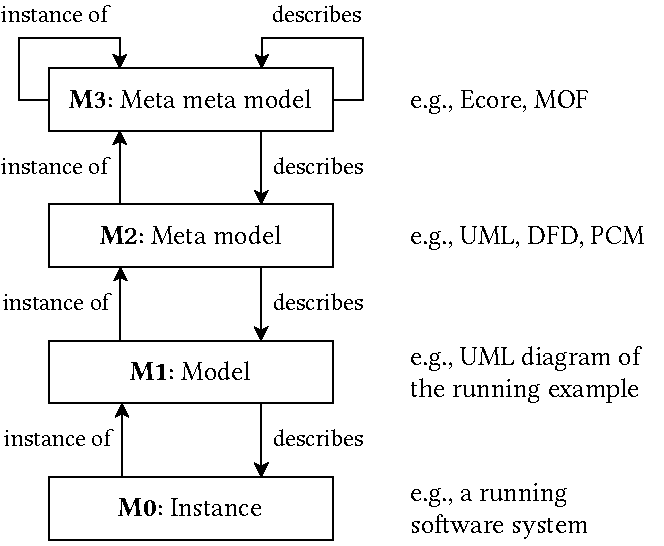
\includegraphics[width=0.65\textwidth]{figures/chapter2/metalevels.pdf}
    \caption{The four meta levels with examples from our domain, based on \textcite{stahl_model-driven_2006}.}
    \label{fig:foundations:metalevels}
\end{figure}

\acf{MDSD} is a concept where models play a central role in the development of software systems \cite{stahl_model-driven_2006}.
Nowadays, using models in software development is common, e.g., as shown by the popularity of the \acf{UML}.
However, compared to only using models for documentation purposes, model-driven approaches give models an equivalent or higher importance than code.
This includes techniques like tailored modeling languages, model transformations, and code generation.
This thesis uses design time models for analysis purposes, which is related to \ac{MDSD}.

\textcite{stachowiak_allgemeine_1973} names three central properties of models: representation, abstraction, and pragmatics.
First, a model represents the modeled entity, e.g., a \ac{UML} diagram can represent the structure or behavior of a real software system.
Second, a model abstracts from the modeled entity, e.g., a \ac{UML} activity diagram does not represent every single line of code.
Third, a model has pragmatics, it follows a purpose.
The models we use are generally about representing a software system in a simplified yet analyzable way.

One of the most important aspects of \ac{MDSD} is meta modeling.
A meta model describes the structure of a model, including available elements, their relationship, and modeling constraints \cite{stahl_model-driven_2006}.
Put simply, a meta model states the rules on how a model has to be constructed.
An example is the \ac{UML} providing many diagram types like activity diagrams, class diagrams, or deployment diagrams.
The meta model itself can be described following the same concept using a meta meta model, which states the rules of the meta model.
Common meta meta models are the \ac{OMG} \acf{MOF} \cite{omg_about_2016} and Ecore from the \acf{EMF} \cite{steinberg_emf_2008}.
Due to the high level of abstraction, these models can describe themselves.
This is visualized in \autoref{fig:foundations:metalevels}.
There, we depict the description and instance relation of all meta levels and show examples from the domain of this thesis, e.g., Ecore, the \ac{UML} meta model, and \ac{UML} models.
This includes the instance level, representing an entity of the real world, e.g., the modeled software system.

\furtherreading{We recommend the comprehensive introduction to \acf{MDSD} by \textcite{stahl_model-driven_2006}.}





\section{Software Architecture}%
\label{sec:foundations:architecture}

As stated in the title of this thesis, this work uses the architectural representation of software systems as a baseline.
Software architecture comprises the \enquote{fundamental concepts or properties of a system in its environment embodied in its elements, relationships, and in the principles of its design and evolution} \cite{international_organization_for_standardization_isoiecieee_2022}, according to the ISO/IEC/IEEE 42010 standard.
Software architecture can be also interpreted as a set of \acfp{ADD} \cite{jansen_architectural_2008,jansen_software_2005}.
Another approach to software architecture is to describe it by its views, e.g., a logical view, or a development view \cite{kruchten_41_1995}.
As discussed in the previous section, we used model-driven techniques.
Here, \acfp{ADL} provide \enquote{means of expression, with syntax and semantics, consisting of a set of representations, conventions, and associated rules intended to be used to describe an architecture} \cite{international_organization_for_standardization_isoiecieee_2022}.
As a meta model for this work, we use the \acf{PCM} \cite{reussner_modeling_2016}, which we describe in more detail in the following.

The Palladio approach \cite{reussner_modeling_2016} enables modeling, simulating, and analyzing software architectures regarding quality dimensions like performance, reliability, or maintainability.
Besides comprehensive tool support \cite{reussner_palladio_2024}, the approach provides a meta model for software architecture, the \ac{PCM} \cite{reussner_palladio_2011,reussner_modeling_2016}.
Palladio builds on the concept of \acf{CBSE}, which divides software architectures into reusable and composable components.
The \ac{PCM} meta model has been used previously in security analysis, e.g., regarding confidentiality \cite{seifermann_architectural_2022}, access control analysis \cite{pilipchuk_architectural_2021}, or attacker propagation \cite{walter_context-based_2023}.
Here, the shared underlying meta model simplifies the reuse of architectural models, which minimizes costs.
The \ac{PCM} is partitioned into five submodels:

\begin{itemize}
    \item The \emph{Component Repository Model} contains components and interfaces.
    The components' behavior is described using \acfp{SEFF} that abstract from the control flow.
    Components can be composed both vertically, and horizontally.
    The repository belongs to the structural viewpoint.
    The inter-component behavior description with \acp{SEFF} belongs to the behavioral viewpoint.
    For instance, components could be the user management or database of an online learning platform.
    \item The \emph{System Model} describes the assembly, i.e., the wiring of the components of the \emph{Component Repository Model}.
    This belongs to the structural viewpoint.
    For instance, the previously introduced user management component could be wired to the database component for the persistence of user data.
    \item The \emph{Execution Environment Model} defines hardware resources and the network.
    These resources represent the deployment locations of components.
    For instance, resources can be an on-premise server or a cloud service.
    \item The \emph{Component Allocation Model} describes the deployment of assembly contexts that represent components from the system model, i.e., shows the allocation of the components in use.
    This model belongs to the deployment viewpoint.
    For instance, the database component can be deployed on-premise.
    \item The \emph{Usage Model} specifies the user interaction with the software system.
    By modeling expected calls to the components, usage scenarios can be expressed.
    For instance, users interact with the user management when registering on the online platform.
\end{itemize}

In sum, the \ac{PCM} enables the system-independent modeling of components and their behavior and of the executing environment.
Furthermore, engineers describe the system-specific assembly context and the allocation context of the components, and also the usage context of the software system.
Based on these submodels, a multitude of simulations can be executed in the Palladio Bench \cite{reussner_palladio_2024}.
For instance, using the information on expected usage scenarios together with the allocation of components, performance bottlenecks can be identified.
For the sake of this thesis, we only focus on confidentiality.
Thus, we build on the \ac{PCM} as comprehensive \ac{ADL} without relating to other analysis approaches of different quality dimensions like performance and reliability.

We choose the \ac{PCM} as foundation of our work due to its maturity, wide adoption, and reception in the community \cite{koziolek_tracing_2022}.
However, we want to stress that the contributions presented in this dissertation can also be realized with other \acp{ADL}, e.g., the \ac{UML}.
Here, using the \ac{PCM} does not represent a \enquote{vendor lock-in}, as its meta models are related to other well-known diagram types like \ac{UML} component diagrams or \ac{UML} activity diagrams.

\furtherreading{\textcite{reussner_modeling_2016} present the Palladio approach in detail.
Additionally, they provide an overview of software architecture as a discipline with a focus on architectural modeling and analysis.}





\section{Data Flow Diagrams}%
\label{sec:foundations:dfd}

\textcite{demarco_structure_1979} introduces \acfp{DFD} to represent software systems \enquote{from the point of view of the data} \cite{demarco_structure_1979}.
By focusing on data flows instead of control flows, the data-oriented analysis of issues within software systems is simplified.
Regarding security analysis, \acp{DFD} represent a simple yet powerful representation of software systems \cite{schneider_how_2024}.
They are used both for documentation and discussion \cite{sion_security_2020,schneider_how_2024}, and also automated analysis \cite{alshareef_precise_2022,seifermann_detecting_2022,canfora_data_1992,berger_automatically_2016,tuma_flaws_2019,tuma_automating_2020}.
Especially regarding confidentiality, the use of \acp{DFD} is expedient, as \enquote{problems tend to follow the data flow, not the control flow} \cite{shostack_threat_2014}.
In the following, we briefly introduce the original syntax of \acp{DFD} \cite{demarco_structure_1979}.
Afterward, we introduce the unified modeling primitives for \acp{DFD} \cite{seifermann_unified_2021}, used throughout this thesis, and the representation of \acp{DFD} as directed graphs \cite{diestel_graph_2017,bang-jensen_digraphs_2009}.

\furtherreading{For a historically relevant, original definition of \acfp{DFD}, we refer to \textcite{demarco_structure_1979}.
To learn more about the fundamentals, see the introduction to graph theory by \textcite{diestel_graph_2017}.}


\subsection{Elements of Data Flow Diagrams}

In describing the conventions of data flow diagrams, \textcite{demarco_structure_1979} states that \enquote{the data flow diagram shows flow of data, not of control} \cite{demarco_structure_1979}.
Resulting from this, loops are excluded from \acp{DFD} as they represent control flow, of which \enquote{the data are unaware of} \cite{demarco_structure_1979}.
The graphical notation of \acp{DFD} comprises four elements:

\begin{itemize}
    \item \emph{Data sources and sinks} are represented by boxes.
    They depict an entity like a person or an organization that is outside of the context of the system under study.
    Examples are the user of a software system or an external data base.
    \item \emph{Processes} are represented by circles.
    They depict the processing or transformation of data within the scope of the system under study.
    Examples are the processing of user input or the calculation of results.
    \item \emph{Files} are represented by straight line.
    They depict internal and temporary repositories of data within the scope of the system under study.
    An example is the temporary storage of intermediate data processing results.
    \item \emph{Data flows} are represented by named arrows.
    They represent data paths or pipelines of data within the software system and connect all other elements.
    Multiple arrows between two elements are possible if the data flow has more than one purpose or type.
    Examples are the flow of data from a source or the flow between two processes.
\end{itemize}

\begin{figure}[b]
    \centering
    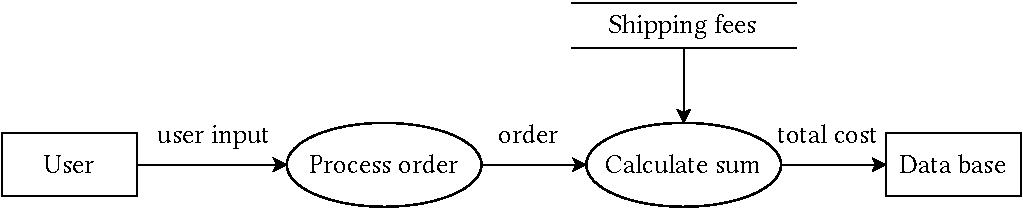
\includegraphics[width=\textwidth]{figures/chapter2/dataflowdiagram.pdf}
    \caption{A \acf*{DFD} showing all four element types in a simplified online shop scenario.}
    \label{fig:foundations:dataflowdiagram}
\end{figure}

\autoref{fig:foundations:dataflowdiagram} shows the \ac{DFD} of a simplified online shop scenario.
The \emph{User} represents a data source, the \emph{Data base} represents a data sink, the \emph{Shipping fees} represent internal storage, and the internal processing represents processes.
All elements are connected by named arrows, i.e., data flows.
The user input comprising an order from the shop is first processed.
Afterward, the total cost of the order is calculated, which includes applying the correct shipping fee.
The result is stored in the data base.
This figure shows several conventions of \textcite{demarco_structure_1979}, e.g., the arrows of files have no description as their purpose is unambiguous.
Inspired by related work \cite{seifermann_architectural_2022}, we use two horizontal lines to represent files throughout this thesis to increase readability.


\subsection{Unified Modeling Primitives}

The \ac{DFD} syntax is simple and easy to understand.
However, this simplicity causes ambiguity, especially regarding security analysis.
\textcite{sion_security_2020} name several weaknesses of \acp{DFD} for security-related analysis:
They lack the means to represent security concepts, lack precision in describing the details of flowing data, and do not express deployment information.
To address this, \textcite{seifermann_unified_2021} present the \emph{unified modeling primitives} of \acp{DFD} by combining multiple notations of security-focussed \ac{DFD} notations from other work \cite{seifermann_data-driven_2019,tuma_flaws_2019}.
We use these primitives in this thesis to represent \acp{DFD}.

\begin{figure}
    \centering
    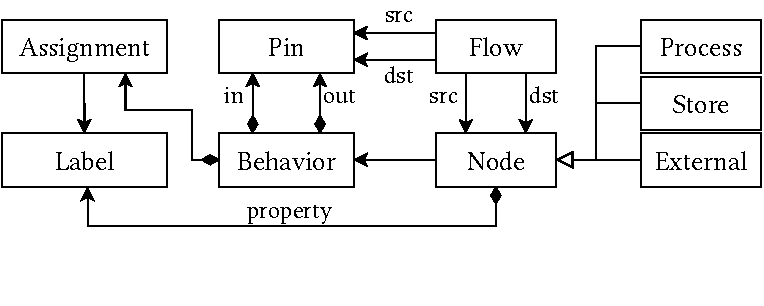
\includegraphics[width=0.85\textwidth]{figures/chapter2/unifiedmodelingprimitives.pdf}
    \caption{Meta model of unified modeling primitives, based on \textcite{seifermann_unified_2021}.}
    \label{fig:foundations:unifiedmodelingprimitives}
\end{figure}

\autoref{fig:foundations:unifiedmodelingprimitives} shows the meta model of the unified modeling primitives.
It comprises the element types known from \acp{DFD} by \textcite{demarco_structure_1979}, i.e., \emph{External} nodes, \emph{Processes}, and internal \emph{Stores}.
These \emph{Nodes} are connected by \emph{Flows}.
To reduce the ambiguity of data flows, \emph{Pins} are used to represent the incoming and outgoing data of a \emph{Node}.
Alternative \emph{Pins} can be used to represent required inputs, e.g., the calculation of the sum in \autoref{fig:foundations:dataflowdiagram} requires both the order and the shipping fees.
Multiple ingoing flows to a single \emph{Pin}, or multiple outgoing flows from a single \emph{Pin} represent alternative flows.
\emph{Pins} are used to decouple the \emph{Behavior} from a \emph{Node}.
A \emph{Behavior} describes the data processing of a node using \emph{Assignments}.
\emph{Assignments} alter \emph{Labels} that represent characteristics of flowing data, e.g., whether data is encrypted or personal.
For instance, the order processing in \autoref{fig:foundations:dataflowdiagram} removes all personal information of the user and only forwards the cost of purchased items, which can be represented using an \emph{Assignment} within the \emph{Behavior} of the \emph{Process}.
This addresses the shortcoming regarding behavior descriptions \cite{sion_security_2020}.
Last, \emph{Labels} are used to describe the properties of \emph{Nodes}, e.g., their deployment.

Using the unified modeling primitives, we can analyze transitive data flows by tracing \emph{Labels} in \acp{DFD}.
The procedure of following \emph{Labels} through the system is called \emph{label propagation} \cite{seifermann_architectural_2022,seifermann_unified_2021,seifermann_detecting_2022}.
To identify confidentiality violations, the propagated \emph{Labels} can be compared to the property \emph{Labels} of a node.
This enables the specification of confidentiality requirements as data flow constraints \cite{hahner_modeling_2021,hahner_domain-specific_2020}.
We reuse conventions for the behavior and constraint description, e.g., the two-headed arrow $\twoheadrightarrow$ represents the forwarding of data in a \ac{DFD}.
The crossed-out arrow $\nrightarrow$ is used to represent a forbidden data flow.
For instance, the data flow constraint of personal data that shall \emph{never flow} to the data base can be written using \emph{Labels} as $\textit{personal} \nrightarrow \textit{database}$.
For a more detailed explanation, see the work of \textcite{seifermann_architectural_2022}, and Boltz~and~Hahner~et.~al~\cite{boltz_extensible_2024}.


\subsection{Directed Acyclic Graphs}

As stated previously, \acp{DFD} use arrows to depict the flow of data.
These arrows represent directed connections between nodes, usually without forming cycles \cite{demarco_structure_1979}.
Thus, \acp{DFD} can be interpreted as graphs where vertices are represented by processes, files, data sources, or data stinks.
The data flows form the edges of the graph.
In graph theory \cite{diestel_graph_2017,bang-jensen_digraphs_2009}, such graphs are referred to as a \acf{DAG}.

A \ac{DAG} is a pair $G = (V, E)$ of sets, where $V$ represents the vertices and $E \subseteq [V]^2$ represents the edges.
We assume that both represent nonempty and finite sets and $V \cap E = \emptyset$.
We write $\abs{G}$ to represent the order of $G$, i.e., the number of its vertices.
Furthermore, we require the graph to be directed and free of cycles.
Note that control flow graphs with cycles can be transformed into acyclic \acp{DFD} \cite{kramer_combining_1994}.
As we use \acp{DAG} only to represent data flows, we do not use the usual notation of an edge that concatenates its vertices name.
Instead of writing \emph{ab} to depict an edge from \emph{a} to \emph{b}, we use the flow syntax of $\flow{a}{b}$.
Besides representing a simple \ac{DFD}, \autoref{fig:foundations:dataflowdiagram} also satisfies the requirements of a \ac{DAG}.
All data flows are directed and there are no cycles with $V = \setted{\var{User}, \var{Process~order}, \var{Calculate~sum}, \var{Shipping~fees}, \var{Data~base}}$ and, for instance, $\setted{\flow{User}{Process~order}, \flow{Process~order}{Calculate~sum}} \subset E$.

In \acp{DAG}, data flows can be represented as strict partial ordering, being irreflexive, asymmetric, and transitive \cite{knuth_art_1997}.
For all $a,b,c \in V$, this means that $\neg (a < a)$, i.e., there is no data flow of a vertex to itself.
Additionally, if $a < b$, i.e., if there is a flow from \emph{a} to \emph{b}, then $\neg (b < a)$, i.e., there is no flow back, which would create a cycle.
Last, data flows are transitive, i.e., if $a < b$ and $b < c$, then trivially also $a < c$.
\autoref{fig:foundations:dataflowdiagram} exemplifies all three properties:
It is irreflexive and asymmetric, without any cyclic flows or flows of data from a vertex to itself.
Last, it shows transitive flows, e.g., the flow from the \emph{User} to the \emph{Data base}.
In sum, \acp{DAG} are a simple yet powerful notation to represent \acp{DFD}.





\section{Summary and Outlook}%
\label{sec:foundations:summary}

In this chapter, we explained the most relevant foundations of this thesis.
This includes the topics of this thesis, i.e., confidentiality, uncertainty, and software architecture.
We briefly repeat the central definitions based on ISO/IEC 27000 and ISO/IEC/IEEE 42010.
Uncertainty is defined as \enquote{the state, even partial, of deficiency of information related to, understanding or knowledge of, an event, its consequence, or likelihood} \cite{international_organization_for_standardization_isoiec_2018}.
Confidentiality is defined as the \enquote{property that information is not made available or disclosed to unauthorized individuals, entities, or processes} \cite{international_organization_for_standardization_isoiec_2018}.
Last, software architecture can be defined as \enquote{fundamental concepts or properties of a system in its environment embodied in its elements, relationships, and in the principles of its design and evolution} \cite{international_organization_for_standardization_isoiecieee_2022}.

Furthermore, we introduced model-driven approaches to software engineering as we build on model-based techniques in our contributions.
Last, we also discussed multiple \ac{DFD} representations: The original definition of \textcite{demarco_structure_1979}, the unified modeling primitives by \textcite{seifermann_unified_2021}, and the representation of \acp{DFD} as \acp{DAG}.
We use all three notations throughout this thesis.
The example of an online shop, briefly introduced in this chapter, is used as a running example in \readingpath{ch:runningexample}.
Afterward, in \readingpath{ch:overview}, we give an overview of the thesis and its contributions, which are based on the aforementioned foundations.





\section{In Simpler Words}%
\label{sec:foundations:simple}

Our research builds on the work of others.
We build on many findings of other researchers from the last decades.
The most important foundations of our work are presented in this chapter.
First, we introduce the topic of uncertainty.
You can think of uncertainty as the opposite of certainty, i.e., the lack of knowledge about something.
For instance, you may not know what you are going to eat tomorrow---you are unsure, or uncertain.
Next, we introduce confidentiality.
Put simply, if I tell you a secret and ask you not to tell it to anyone else, I ask for confidentiality.
This confidentiality is especially important in software systems that handle large amounts of sensitive data.

We also introduce model-driven approaches to software development and software architecture, known as \acf{MDSD}.
Models can be thought of as diagrams of software systems that show, for example, the structure of a system.
In this thesis, these diagrams are central to our way of thinking about software systems.
We thereby focus on the software architecture, i.e., a higher abstraction of the system under study.
We are not interested in every single line of code but we focus on the bigger questions of how the system is constructed and deployed.

Last, we discuss \acfp{DFD}, as we are especially interested in the confidentiality of data.
Here, we present different notations of such diagrams that differ in their nature and complexity.
For instance, we refer to the original definition by \textcite{demarco_structure_1979} from 1979, and a more recent notation by \textcite{seifermann_unified_2021}.
We also explain a more formal way to draw such diagrams, called \acfp{DAG}.
It is important for us to have appropriate means to express data flows, as the remainder of this thesis will build on them.
